\chapter{Ramsey Theory} \label{Ch6:CH}
\thispagestyle{empty}

The Ramsey numbers of \Cref{Ch2:CH} asked how large a complete graph, or hypergraph, must be before every colouring of its edges is forced to contain a monochromatic clique. This chapter asks the same question of structures that are not graphs at all, and what is forced is no longer a clique: in the integers it is an arithmetic progression, which is van der Waerden's theorem, and in the hypercube $[n]^d$ it is a combinatorial line, which is the Hales--Jewett theorem. Both are proved by the same device, colour-focusing, and the second contains the first and a good deal more besides. We close with the complete graph on $\N$ itself, where Ramsey's theorem is easier than in the finite case and where one of its finite consequences turns out to lie beyond Peano arithmetic.

\section{Van der Waerden's Theorem}

This chapter is motivated by the following question: if I $r$-colour the natural numbers $\N$, must I be able to find arbitrarily long monochromatic arithmetic progressions?

\begin{boxdefinition}[van der Waerden's Number]
    For $k, r \in \N$, the \textbf{van der Waerden number for $k$ and $r$}, denoted $\VW(k, r)$, is the least $N$ such that any $r$-colouring of $[N]$ admits a $k$-term monochromatic arithmetic progression.
\end{boxdefinition}

We will eventually show the following.

\begin{boxtheorem}[van der Waerden's Theorem] \label{Ch6:Thm:Van_Der_Waerden}
    For all $k, r \in \N$, $\VW(k, r)$ exists.
\end{boxtheorem}

$\VW(2, r) = r + 1$ is fairly straightforward. But what about $\VW(3, 2)$?

\subsection{Colour-Focusing}

% The seven provenance markers of the 30 September lecture below were carried over from the author's local copy of it (Local_Collective/lectures_28_30_sept.tex), which the Overleaf copy had dropped.
We can show that $\VW(3, 2) \geq 9$, because of the colouring
% [FILLED] the colours of $1, \ldots, 8$ are the standard extremal colouring, supplied here as the photo of the board does not show them
\begin{align*}
    \textcolor{red!75!black}{1} \quad \textcolor{red!75!black}{2} \quad \textcolor{blue!70!black}{3} \quad \textcolor{blue!70!black}{4} \quad \textcolor{red!75!black}{5} \quad \textcolor{red!75!black}{6} \quad \textcolor{blue!70!black}{7} \quad \textcolor{blue!70!black}{8} \quad 9
\end{align*}
where the minute you hit $9$ you get a monochromatic AP: $1, 5, 9$ if $9$ is red, and $7, 8, 9$ if $9$ is blue. (The choices previously were to try and minimise the chance of getting a $3$-term AP.)

We can also show that $\VW(3, 2) \leq 325$. How?

Write out blocks of five as follows:

\begin{figure}[h] % Note: This figure was generated by Claude
    \centering
    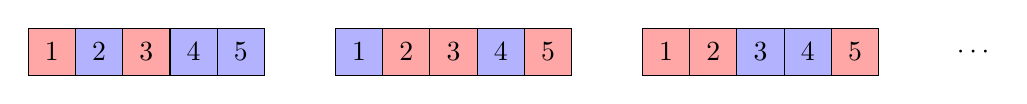
\begin{tikzpicture}[scale = 0.6]
        \foreach \b/\cols in {0/{red!35, blue!30, red!35, blue!30, blue!30}, 1/{blue!30, red!35, red!35, blue!30, red!35}, 2/{red!35, red!35, blue!30, blue!30, red!35}}{
            \foreach \c [count = \i] in \cols {
                \pgfmathsetmacro{\xpos}{6.5 * \b + \i - 1}
                \filldraw[fill = \c, draw = black] (\xpos, 0) rectangle ++(1, 1);
                \node at (\xpos + 0.5, 0.5) {$\i$};
            }
        }
        \node at (20, 0.5) {$\cdots$};
    \end{tikzpicture}
\end{figure}

(This is meant to represent a sequence of consecutive numbers, so the second box should really contain $6, 7, 8, 9, 10$, and so on. But this notation will prove convenient.)

We will essentially discover that when we have $65$ such boxes, any $2$-colouring of this sequence admits a monochromatic $3$-term AP.

Fix a $2$-colouring of this sequence. Notice that in any block of five, there is some $3$-term AP such that the first two terms are monochromatic. (Indeed, this is what motivates the choice of \textit{five} in the first place.)

We have a total of $2^5$ ways of colouring a block of five, so if we write down a total of $33 = 2^5 + 1$ blocks (which, in the worst case, consists of a block with each colour configuration, and then one more), we can always find two identically coloured blocks. Say these are the $i$th and the $j$th, with $i < j \leq 33$. Let $a, a + d, a + 2d \in \set{1, 2, 3, 4, 5}$ be the positions of their $3$-term AP, with $a$ and $a + d$ red, say.\footnote{Hence the notational convenience of using the same numbers, $1, 2, 3, 4, 5$, for each block.} If $a + 2d$ is also red, we're done, so suppose it is blue.

The intuition is to build an ``AP of blocks'' and use the next term after $i$ and $j$ to obtain the desired monochromatic $3$-term AP. Indeed, if we start at block $i$, this AP looks like $i + \ell (j - i)$. Going to the $\ell = 2$ term should give us the $(2j - i)$th block. Let's now show that this works.

Write $D = 5(j - i)$ for the distance between the two blocks, so that the $k$th element of block $j$ is exactly $D + (\text{the $k$th element of block $i$})$. In the $(2j - i)$th block, the $k$th element is exactly $D$ away from the $k$th element of block $j$. Now denote by $x$ the $(a + 2d)$th element of the $(2j - i)$th block.
\begin{description}
    \item[\underline{$x$ is red.}] Then position $a$ of block $i$, position $a + d$ of block $j$ and $x$ form a red AP with difference $D + d$.
    \item[\underline{$x$ is blue.}] Then position $a + 2d$ of blocks $i$, $j$ and $2j - i$ form a blue AP with difference $D$. (Remember, blocks $i$ and $j$ are coloured identically, and since the $(a + 2d)$th element of block $j$ is blue, so is that of $i$.)
\end{description}
Since $2j - i \leq 2 \cdot 33 - 1 = 65$, it suffices to have $65$ blocks of five, ie, $5 \cdot 65 = 325$ numbers.

We will now apply this technique to find a general upper-bound for van der Waerden numbers, and thereby, show they always exist (ie, prove van der Waerden's theorem).

We want to emphasise the concept of \textit{colour-focusing}: in our previous example, we saw that there were two APs that agreed at the last term, that were monochromatic until that one last ``focus'' term was coloured. That colouring would extend one of them but not the other. We thus make the following definition.

% [CORRECTED] was: each AP is monochromatic, except (possibly) at the $k$th term; all the APs have a common $k$th term (the focus point) --- the focus point is now the $(k + 1)$th term, so that the monochromatic AP in the definition of $\CF$ has one more term than the monochromatic part of each colour-focused AP
\begin{boxdefinition}[Colour-Focused APs]
    A collection of $k$-term APs is \textbf{colour-focused} if the following both hold:
    \begin{itemize}
        \item each AP is monochromatic
        \item all the APs have a common $(k + 1)$th term
    \end{itemize}
    The common $(k + 1)$th term of a family of colour-focused APs is called their \textbf{focus point}.
\end{boxdefinition}

The focus point could be the same colour as one of the APs, but it does not have to be. For our purposes, we will be interested in colour-focused APs that are different colours.

Let's now try and repeat the $\VW(3, 2)$ argument to find an upper-bound for $\VW(3, 3)$.

Divide the natural numbers into blocks of $7$. Again, our choice is motivated by the pigeonhole principle: for any $3$-colouring of all the numbers, any $7$-block admits a $3$-term AP such that the first $2$ terms are monochromatic.

\begin{figure}[H]
    \centering
    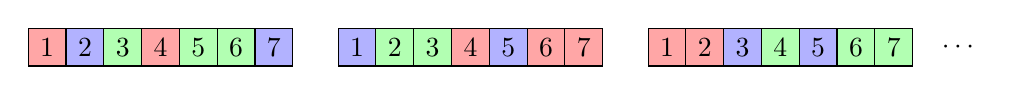
\begin{tikzpicture}[scale = 0.48]
        \foreach \b/\cols in {0/{red!35, blue!30, green!30, red!35, green!30, green!30, blue!30}, 1/{blue!30, green!30, green!30, red!35, blue!30, red!35, red!35}, 2/{red!35, red!35, blue!30, green!30, blue!30, green!30, green!30}}{
            \foreach \c [count = \i] in \cols {
                \pgfmathsetmacro{\xpos}{8.2 * \b + \i - 1}
                \filldraw[fill = \c, draw = black] (\xpos, 0) rectangle ++(1, 1);
                \node at (\xpos + 0.5, 0.5) {$\i$};
            }
        }
        \node at (24.6, 0.5) {$\cdots$};
    \end{tikzpicture}
\end{figure}

We have a total of $3^7$ ways of colouring a block, so if we write down $3^7 + 1 = 2188$ blocks, there are bound to be two that are identically coloured. As before, if we double this number and subtract one, ie, if we have $2\parenth{3^7 + 1} - 1 = 4375$ blocks, then we are guaranteed to have two colour-focused APs with a focus point.

The problem is that this focus point could take \textit{three} values, but as we only have two monochromatic APs, if it takes the colour not taken by the two APs, we do not have a monochromatic $3$-term AP.

What we have shown above is that if we have a total of $4375$ blocks, that is, $7 \cdot 4375$ numbers, we are guaranteed to have two APs with a shared focus point, which may or may not complete them.

To get three colour-focused APs, we need to ``go up one level'' and treat blocks of $7 \cdot 4375 = 30625$ numbers the way we treated blocks of $7$ to get two colour-focused APs. By the above, each such block contains either a monochromatic $3$-term AP, in which case we're done, or two colour-focused APs of different colours, say red and blue, whose focus point is green. There are $3^{30625}$ ways of colouring a $30625$-block, so among $3^{30625} + 1$ of them, two are identically coloured, say the $i$th and the $j$th. Write $\Delta = 30625(j - i)$, and let $y$ be the element of the $(2j - i)$th block in the same position as the focus point. We now have three APs heading for $y$:
\begin{itemize}
    \item the red AP, with its first term taken from block $i$ and its second from block $j$;
    \item the blue AP, likewise;
    \item the focus point of block $i$ followed by the focus point of block $j$, both green.
\end{itemize}

\begin{figure}[H] % Note: this diagram was generated by Claude
    \centering
    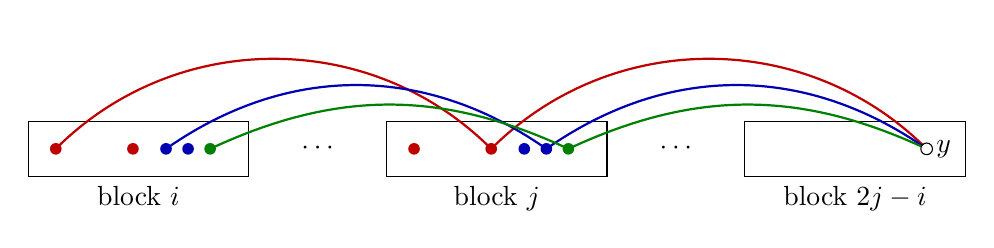
\begin{tikzpicture}[scale = 0.7]
        \foreach \x/\lab in {0/i, 6.5/j, 13/2j - i}{
            \draw (\x, 0) rectangle ++(4, 1);
            \node[below] at (\x + 2, 0) {block $\lab$};
        }
        \node at (5.25, 0.5) {$\cdots$};
        \node at (11.75, 0.5) {$\cdots$};
        \draw[red!75!black, thick] (0.5, 0.5) to[bend left = 45] (8.4, 0.5) to[bend left = 45] (16.3, 0.5);
        \draw[blue!70!black, thick] (2.5, 0.5) to[bend left = 35] (9.4, 0.5) to[bend left = 35] (16.3, 0.5);
        \draw[green!50!black, thick] (3.3, 0.5) to[bend left = 25] (9.8, 0.5) to[bend left = 25] (16.3, 0.5);
        \foreach \x in {0, 6.5}{
            \foreach \p/\c in {0.5/red!75!black, 1.9/red!75!black, 2.5/blue!70!black, 2.9/blue!70!black, 3.3/green!50!black}{
                \fill[\c] (\x + \p, 0.5) circle (3pt);
            }
        }
        \filldraw[fill = white, draw = black] (16.3, 0.5) circle (3pt) node[right] {$y$};
    \end{tikzpicture}
\end{figure}

Each of these is monochromatic, they have different colours, and each continues to $y$: if $p, q$ is an AP in block $i$ whose next term is the focus point $f$, then $p$ and $q + \Delta$ form an AP whose next term is $f + 2\Delta = y$. So these are three colour-focused APs of different colours, and whatever the colour of $y$, it completes one of them to a monochromatic $3$-term AP. As before, it suffices to have $2\parenth{3^{30625} + 1} - 1$ blocks of $30625$ numbers, so
\begin{align*}
    \VW(3, 3) \leq 30625 \cdot \parenth{2 \cdot 3^{30625} + 1}
\end{align*}

Not only have we found a bound on $\VW(3, 2)$ and $\VW(3, 3)$, we've also shown they \textit{exist}. We can actually use the strategy above to prove van der Waerden's Theorem (\Cref{Ch6:Thm:Van_Der_Waerden}).

\subsection{Colour-Focus Numbers}

First, a general definition.

% [CORRECTED] was: $s$ colour-focused $k$-term APs --- the focus can only be trapped if the APs have different colours (cf. the remark after the definition of colour-focused APs) and the focus point lies in $[N]$, so that it is coloured
\begin{boxdefinition}[Colour-Focus Number]
    For $k, r, s$ with $s \le r$, define the \textbf{colour-focus number} $\CF(k, r, s)$ to be the least $N$ such that any $r$-colouring of $[N]$ has either a monochromatic $(k + 1)$-term AP or $s$ colour-focused $k$-term APs of different colours, with focus point in $[N]$.
\end{boxdefinition}

We can bound van der Waerden numbers above by colour-focus numbers as follows.

\begin{boxlemma}\label{Ch6:Lemma:VW_le_CF}
    For all $k, r \in \N$,
    \begin{align*}
        \VW(k, r) \le \CF(k-1, r, r)
    \end{align*}
\end{boxlemma}
\begin{proof}
    Let $N = \CF(k-1, r, r)$. We need to show that any $r$-colouring of $[N]$ contains a $k$-term monochromatic arithmetic progression. But by definition of the colour-focus number, either $[N]$ admits a $k$-term monochromatic arithmetic progression (in which case we're done) or $r$ colour-focused $(k - 1)$-term arithmetic progressions. As we argued above, if there are $r$ such APs, then the focus must complete one of them, as we are $r$-colouring. So again we're done.
\end{proof}

We now prove a recursive bound on the colour-focus numbers.
% [CORRECTED] the proof below was re-indexed to match: a $(k - 1)$-term AP of blocks became a $k$-term one, $j \leq k - 1$ became $j \leq k$, and the focus block $B_{a + (k - 1)d}$ became $B_{a + kd}$; the sentence on the colour of the AP of focus points was added, as was ``of different colours'' in its first and last paragraphs, and ``for $k \geq 2$'' in the footnote

% [CORRECTED] was: For all $k, r, s \in \N$, with $\VW\of{k - 1, \cdot}$ --- $\CF(k, r, s - 1)$ needs $s \geq 2$, $\CF(k, r, s)$ needs $s \leq r$, and stretching APs with $k$ monochromatic terms needs $k$ identically coloured blocks, ie $\VW\of{k, \cdot}$
\begin{boxlemma}\label{Ch6:Lemma:CF_Recursion}
    For all $k, r, s \in \N$ with $2 \leq s \leq r$,
    \begin{align*}
        \CF(k, r, s)
        \leq \CF(k, r, s - 1) \cdot 2 \VW\of{k, r^{\CF\of{k, r, s - 1}}}
    \end{align*}
\end{boxlemma}
\begin{proof}
    Fix an $N \in \N$ and an $r$-colouring of $[N]$. Let $C = \CF\of{k, r, s - 1}$. Consider blocks in $[N]$ of length $C$. If any of them contains a $(k + 1)$-term monochromatic arithmetic progression, we're done, so assume that they all contain $(s - 1)$ $k$-term colour-focused arithmetic progressions of different colours. As they are all of length $C$, they must all have one property or the other.
    
    Each block can be coloured in one of $r^C$ ways. If we took $\VW\of{k, r^C}$ many blocks, say $B_1, \ldots, B_{\VW\of{k, r^C}}$, by definition of $\VW$, we would be able to find a $k$-term ``arithmetic progression of blocks''
    \begin{align*}
        B_{a}, B_{a + d}, B_{a + 2d}, \ldots, B_{a + (k - 1)d}
    \end{align*}
    that are all identically coloured.\footnote{We can ``code APs of blocks as APs'', and in this coding, a sequence of numbers being monochromatic translates to blocks being identically coloured.} If we take $2\VW\of{k, r^C}$ blocks\footnote{For $k \geq 2$, $2\VW\of{k, r^{\CF(k, r, s - 1)}} - 1$ would suffice, and we can even get tighter bounds, but the expression looks nicer without the ${} - 1$.}, we also have the focus block $B_{a + kd}$.

    What are some properties of this focus block? We know that it may not be coloured identically to the others in the AP of blocks. However, every block (APs and focus alike) has exactly $C$ elements, so each block contains $(s - 1)$ $k$-term colour-focused APs. Then, the families of APs that looks like ``the $j$th term of the $j$th block'', I get an AP with a focus point in $B_{a + kd}$. Ie, suppose my $(s - 1)$ $k$-term APs are denoted $\parenth{x^i_j}_{1 \leq j \leq k}$ for $1 \leq i \leq s - 1$, then I can build new APs $\parenth{y^i_j}_{1 \leq j \leq k}$ where for each $i$ in my family, I define $y^i_j$ to be the instance of $x^i_j$ living in the $j$th block $B_{a + (j - 1)d}$. This gives me $(s - 1)$ colour-focused APs in my set of numbers from the $2\VW\of{k, r^C}$ blocks (the focus point being the element of the focus block occupying the position of the focus points in the other blocks). Moreover, when I take the AP consisting of all the focus points, I get yet another AP with the same focus point as the $\parenth{y^i_j}$. Its colour is different from theirs: the $\parenth{y^i_j}$ have the colours of the $\parenth{x^i_j}$, and if the focus point of $B_a$ had the same colour as one of the $\parenth{x^i_j}$, the two together would form a monochromatic $(k + 1)$-term AP, which we have ruled out. Thus, I get a total of $s$ colour-focused APs.
    
    \begin{figure}[h] % Note: this diagram was generated by Claude
        \centering
        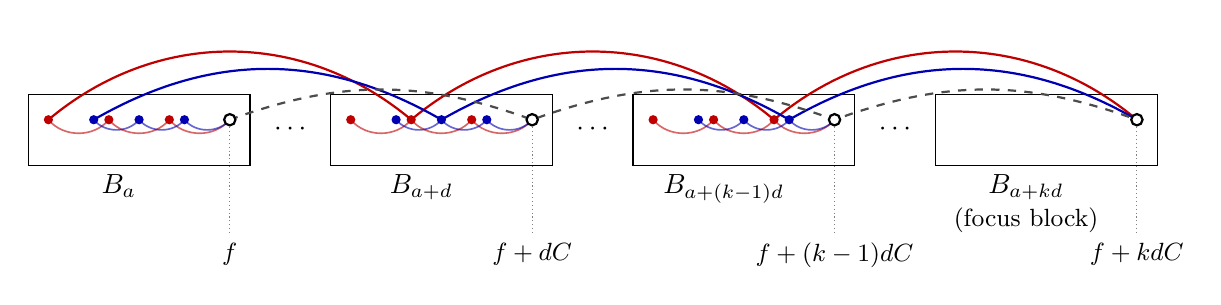
\begin{tikzpicture}[scale = 0.64]
            \foreach \x/\lab in {0/a, 6/a + d, 12/a + (k - 1)d, 18/a + kd}{
                \draw (\x, 0) rectangle ++(4.4, 1.4);
                \node[below] at (\x + 1.8, 0) {$B_{\lab}$};
            }
            \node at (5.2, 0.7) {$\cdots$};
            \node at (11.2, 0.7) {$\cdots$};
            \node at (17.2, 0.7) {$\cdots$};
            \node[below] at (19.8, -0.65) {\small (focus block)};
            % inside each identically coloured block: the s - 1 colour-focused APs, running into that block's focus point
            \foreach \x in {0, 6, 12}{
                \draw[red!75!black, semithick, opacity = 0.6] (\x + 0.4, 0.9) to[bend right = 50] (\x + 1.6, 0.9) to[bend right = 50] (\x + 2.8, 0.9) to[bend right = 50] (\x + 4, 0.9);
                \draw[blue!70!black, semithick, opacity = 0.6] (\x + 1.3, 0.9) to[bend right = 50] (\x + 2.2, 0.9) to[bend right = 50] (\x + 3.1, 0.9) to[bend right = 50] (\x + 4, 0.9);
            }
            % across blocks: the stretched APs, and the AP of focus points
            \draw[red!75!black, thick] (0.4, 0.9) to[bend left = 40] (7.6, 0.9) to[bend left = 40] (14.8, 0.9) to[bend left = 40] (22, 0.9);
            \draw[blue!70!black, thick] (1.3, 0.9) to[bend left = 30] (8.2, 0.9) to[bend left = 30] (15.1, 0.9) to[bend left = 30] (22, 0.9);
            \draw[black!70, thick, dashed] (4, 0.9) to[bend left = 20] (10, 0.9) to[bend left = 20] (16, 0.9) to[bend left = 20] (22, 0.9);
            \foreach \x in {0, 6, 12}{
                \foreach \p/\c in {0.4/red!75!black, 1.6/red!75!black, 2.8/red!75!black, 1.3/blue!70!black, 2.2/blue!70!black, 3.1/blue!70!black}{
                    \fill[\c] (\x + \p, 0.9) circle (2.6pt);
                }
            }
            % the focus points, hollow, labelled underneath the diagram
            \foreach \x/\lab in {0/f, 6/f + dC, 12/f + (k - 1)dC, 18/f + kdC}{
                \filldraw[fill = white, draw = black, thick] (\x + 4, 0.9) circle (3.2pt);
                \draw[black!50, densely dotted] (\x + 4, 0.75) -- (\x + 4, -1.35);
                \node[below] at (\x + 4, -1.35) {\small $\lab$};
            }
        \end{tikzpicture}
    \end{figure}

    The total number of elements living in my $2\VW\of{k, r^C}$ blocks is $C \cdot 2\VW\of{k, r^C}$. So effectively, when $N = C \cdot 2\VW\of{k, r^C}$, any $r$-colouring of $[N]$ admits either a $(k + 1)$-term monochromatic AP or $s$ colour-focused $k$-term APs of different colours. Thus, this value of $N$ is an upper-bound on $\CF\of{k, r, s}$.
\end{proof}

We can use our recursive bound on colour-focus numbers to prove that colour-focus numbers always exist\footnote{Maybe you need to choose $k, r, s$ so that $\CF(k, r, s)$ actually makes sense, but we won't split hairs about this.}. This ultimately tells us that van der Waerden numbers also always exist.

\begin{boxtheorem}
    $\CF(k, r, s)$ always exists.
\end{boxtheorem}
\begin{proof}
    % [CORRECTED] the base case below gained the pigeonhole step, needed now that colour-focused APs must have different colours
    Proceed by induction on $k$, keeping $r$ and $s$ generic\footnote{In Lean this would be \lstinline|induction k generalizing r s|.}. When $k = 1$, the result is trivial, because no matter the value of $r$ or $s$, if we consider the set $[s + 1]$, we can always find either a $2$-term monochromatic AP (ie, two numbers with the same colour) or $s$ $1$-term monochromatic colour-focused APs (ie, $s + 1$ numbers with distinct colours).

    Now fix $k$ and assume $\CF(k, r, s)$ exists for all $r, s$. We want to show that $\CF(k + 1, r, s)$ also exists for all $r, s$. We proceed by induction on $s$.

    $\CF(k + 1, r, 1)$ certainly always exists. In general, $\CF(a, b, 1)$ exists iff there is some $N \in \N$ such that any $b$-colouring of $[N]$ admits a monochromatic $a$-term AP. Take $N \geq \CF(k, r, r)$ (which exists by the induction hypothesis on $k$). Then either $[N]$ admits a $(k + 1)$-term monochromatic AP (in which case we're done) or $[N]$ admits $r$ colour-focused $k$-term APs (in which case the focus point extends one of them to a monochromatic $(k + 1)$-term AP, as there are precisely $r$ of them).

    % [CORRECTED] was: $\VW\of{k, \cdot}$ and $\CF\of{k - 1, \cdot, \cdot}$ below --- these follow the recursive bound's $\VW\of{k + 1, \cdot}$, and $\CF\of{k, \cdot, \cdot}$ is exactly the induction hypothesis on $k$
    Now fix $s$ and suppose $\CF(k + 1, r, s)$ exists for all $r$. Then by \Cref{Ch6:Lemma:CF_Recursion,Ch6:Lemma:VW_le_CF}, we know
    \begin{align*}
        \CF\of{k + 1, r, s + 1}
        &\leq \CF\of{k + 1, r, s} \cdot 2 \VW\of{k + 1, r^{\CF\of{k + 1, r, s}}} \\
        &\leq \CF\of{k + 1, r, s} \cdot 2 \CF\of{k, r^{\CF\of{k + 1, r, s}}, r^{\CF\of{k + 1, r, s}}}
    \end{align*}
    The above colour-focus numbers both exist by the induction hypotheses on $k$ and $s$, finishing the induction.
\end{proof}

\Cref{Ch6:Thm:Van_Der_Waerden} (van der Waerden's theorem) is an immediate corollary.

\subsection{A Lower Bound from the Local Lemma}

The bounds above are enormous, and it is worth recording what is known from below, which comes from the \Lovasz{} local lemma (\Cref{Ch5:Thm:LLL}): it is the benchmark against which every upper bound in this chapter should be read.

% Not from the lecture: the lecture of 7 October quoted this bound as already shown, ``using the Lovasz Local Lemma'', and no earlier lecture in these notes shows it (chapter 5 states the lemma and proves nothing with it yet). The statement and proof were supplied in answer to the author's ``when? where? how?''; the symmetric form of the local lemma that the proof uses is not in chapter 5 either, so it is derived inline by taking every $x_A$ equal.
\begin{boxproposition} \label{Ch6:Prop:VW_Lower_Bound}
    For all $k \geq 2$,
    \begin{align*}
        \VW\of{k, 2} > \frac{(k - 1) \, 2^{k - 1}}{e k^2}
    \end{align*}
    In particular, $\VW\of{k, 2} = \Omega\of{\frac{2^k}{k}}$.
\end{boxproposition}
\begin{proof}
    Let $N = \floor{\frac{(k - 1) 2^{k - 1}}{e k^2}} + 1$. It suffices to find a $2$-colouring of $[N]$ with no monochromatic $k$-term arithmetic progression, as then $\VW(k, 2) > N$. If $N < k$ there is nothing to find, since $[N]$ has no $k$-term progressions at all, so assume $N \geq k$.

    Colour $[N]$ red or blue uniformly and independently at random. For each $k$-term arithmetic progression $P \ssq [N]$, let $A_P$ be the event that $P$ is monochromatic, so that $\Pr\of{A_P} = 2^{1 - k}$. $A_P$ is determined by the colours of the points of $P$ alone, so joining $A_P$ to $A_Q$ exactly when $P$ and $Q$ share a point gives a dependency graph. A progression through a given point is determined by its common difference, which is at most $\frac{N - 1}{k - 1}$, and by the position of the point in it, so a point lies in at most $\frac{k (N - 1)}{k - 1}$ progressions, and $A_P$ has at most
    \begin{align*}
        D = \frac{k^2 (N - 1)}{k - 1} - 1 \geq 1
    \end{align*}
    neighbours. Take $x_A = \frac{1}{D + 1}$ for every event $A$. Then, for every $P$,
    \begin{align*}
        x_{A_P} \prod_{A_Q \sim A_P} \parenth{1 - x_{A_Q}}
        \geq \frac{1}{D + 1} \parenth{1 - \frac{1}{D + 1}}^{D}
        \geq \frac{1}{e \parenth{D + 1}}
        = \frac{k - 1}{e k^2 (N - 1)}
        \geq 2^{1 - k}
        = \Pr\of{A_P}
    \end{align*}
    using $\parenth{1 + \frac{1}{D}}^D \leq e$ for the second inequality and $N - 1 \leq \frac{(k - 1) 2^{k - 1}}{e k^2}$ for the last. So \Cref{Ch5:Thm:LLL} applies, and with positive probability no $A_P$ occurs: some $2$-colouring of $[N]$ has no monochromatic $k$-term arithmetic progression.
\end{proof}

\section{The Hales--Jewett Theorem}

Van der Waerden's theorem is about progressions in the integers. The Hales--Jewett theorem strips the arithmetic away and keeps only the combinatorics of the colour-focusing argument, and it is the stronger result: at the end of this section it will give van der Waerden's theorem back, and other things with it.

\subsection{Combinatorial Lines}

Combinatorial lines are what Hales--Jewett replaces arithmetic progressions with, and the hypercube $[n]^d$---the set of strings of length $d$ over the alphabet $[n]$---is where they live.

% [FILLED] definition supplied; the lecture used ``line'' without defining it, and the arguments below need the template
\begin{boxdefinition}[Combinatorial Line]
    Fix $n, d \in \N$ and a symbol $x \notin [n]$. A \textbf{template} is a string $\sigma \in \parenth{[n] \cup \set{x}}^d \setminus [n]^d$, ie, one in which $x$ occurs at least once; the coordinates at which $\sigma$ is $x$ are its \textbf{active coordinates}, and the others are \textbf{fixed}. For $i \in [n]$, write $\sigma(i) \in [n]^d$ for the string obtained from $\sigma$ by replacing every $x$ by $i$. The \textbf{combinatorial line} with template $\sigma$ is
    \begin{align*}
        L_\sigma = \set{\sigma(1), \sigma(2), \ldots, \sigma(n)}
    \end{align*}
    and $\sigma(n)$ is its \textbf{last point}. We will usually just say \textbf{line}.
\end{boxdefinition}

In $[3]^2$, for instance, the templates $x1$, $2x$ and $xx$ give two lines parallel to the axes and the main diagonal, whereas the anti-diagonal $\set{13, 22, 31}$ is a line in the geometric sense but not a combinatorial one, since its two coordinates move in opposite directions. The number we are after is the dimension that forces a monochromatic line.

\begin{boxdefinition}[Hales-Jewett Number]
    For all $n, r \in \N$, define $\HJ(n, r)$ to be the smallest number $d$ such that any $r$-colouring of the hypercube $[n]^d$ has a monochromatic line.
\end{boxdefinition}

As with van der Waerden's numbers, we will eventually show that these always exist.

\begin{boxtheorem}[Hales--Jewett Theorem] \label{Ch6:Thm:Hales_Jewett}
    For all $n, r \in \N$, $\HJ(n, r)$ exists.
\end{boxtheorem}

\subsection{Colour-Focused Lines}

Colour-focusing works for lines exactly as it did for arithmetic progressions.

\begin{boxdefinition}[Colour-Focused Lines]
    Given combinatorial lines $L_1, L_2, \ldots, L_s$, they are \textbf{colour-focused} if their last points coincide and each is monochromatic (in a distinct colour) on all but the last point.
\end{boxdefinition}

For example, draw $[3]^2$ as a grid, with the first coordinate running left to right and the second bottom to top. In the colouring below, the top row, the right-hand column and the diagonal are three colour-focused lines: each is monochromatic on its first two points, in orange, purple and green respectively, and all three end at the top-right point, which is their focus. Whatever colour that point gets, it completes one of them; here it is orange, and the top row is a monochromatic line.

\begin{figure}[H]
    \centering
    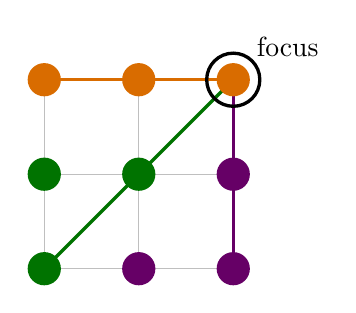
\begin{tikzpicture}[scale = 1.2]
        \draw[gray!50] (1, 1) grid (3, 3);
        \draw[orange!85!black, very thick] (1, 3) -- (3, 3);
        \draw[violet!80!black, very thick] (3, 1) -- (3, 3);
        \draw[green!45!black, very thick] (1, 1) -- (3, 3);
        \foreach \x/\y/\c in {1/3/orange!85!black, 2/3/orange!85!black, 3/3/orange!85!black, 1/2/green!45!black, 2/2/green!45!black, 3/2/violet!80!black, 1/1/green!45!black, 2/1/violet!80!black, 3/1/violet!80!black}{
            \fill[\c] (\x, \y) circle (5pt);
        }
        \draw[black, very thick] (3, 3) circle (8pt);
        \node[above right = 5pt] at (3, 3) {focus};
    \end{tikzpicture}
\end{figure}

\begin{boxdefinition}[Focused Hales-Jewett Number]
    $\FHJ(n, r, s)$ is the minimum $d$ such that any $r$-colouring of $[n]^d$ has $s$ colour-focused lines or a monochromatic line.
\end{boxdefinition}

We can see that
% [FILLED] the display was boxed as a lemma and the one-line proof supplied; the lecture said ``we can see that''
\begin{boxlemma} \label{Ch6:Lemma:HJ_le_FHJ}
    For all $n, r \in \N$,
    \begin{align*}
        \HJ(n, r) \le \FHJ(n, r, r)
    \end{align*}
\end{boxlemma}
\begin{proof}
    Let $d = \FHJ(n, r, r)$ and fix an $r$-colouring of $[n]^d$. If it has a monochromatic line we are done. Otherwise it has $r$ colour-focused lines, of $r$ distinct colours, with a common last point. That point has one of the $r$ colours, so it completes the line of that colour to a monochromatic one.
\end{proof}

We will also show
% [FILLED] the display was boxed as a lemma, with ``$2 \leq s \leq r$'' added so that $\FHJ(n, r, s - 1)$ makes sense (cf. the recursive bound on colour-focus numbers); the author's setup of the proof is kept and the argument completed from where it broke off
\begin{boxlemma} \label{Ch6:Lemma:FHJ_Recursion}
    For all $n, r, s \in \N$ with $2 \leq s \leq r$,
    \begin{align*}
        \FHJ(n, r, s) \le \FHJ(n, r, s - 1) + \HJ\of{n - 1, r^{n^{\FHJ(n, r, s - 1)}}}
    \end{align*}
\end{boxlemma}
\begin{proof}
For this argument, denote $\FHJ(n, r, s - 1)$ by $D_2$ and $\HJ\of{n - 1, r^{n^{\FHJ(n, r, s - 1)}}}$ by $D_1$. (The letters are apt because these are dimensions.) We show essentially that $\FHJ(n, r, s) \le D_2 + D_1$ and note that $D_1 = \HJ\of{n - 1, r^{n^{D_2}}}$.

% [CORRECTED] was: ``contains $s$ colour-focused lines.'' --- the definition of $\FHJ$ has two alternatives, and a colouring with a monochromatic line need not have $s$ colour-focused lines of distinct colours (a constant colouring has at most one)
The inequality is essentially saying ``any $r$-colouring of the $[n]^{D_1 + D_2}$ cube contains $s$ colour-focused lines or a monochromatic line.''

A point in my cube has coordinates

\begin{figure}[H]
    \centering
    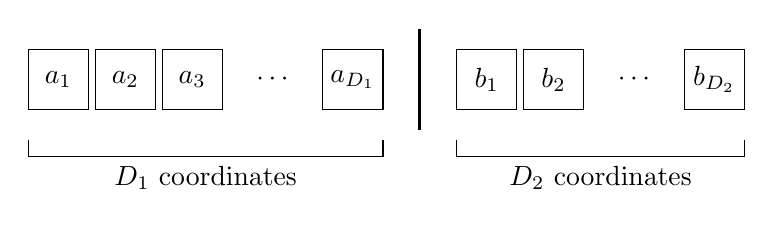
\begin{tikzpicture}[scale = 0.85]
        \foreach \x/\lab in {0/a_1, 1/a_2, 2/a_3, 4.4/a_{D_1}}{
            \draw (\x, 0) rectangle ++(0.9, 0.9);
            \node at (\x + 0.45, 0.45) {$\lab$};
        }
        \node at (3.65, 0.45) {$\cdots$};
        \draw[very thick] (5.85, -0.3) -- (5.85, 1.2);
        \foreach \x/\lab in {6.4/b_1, 7.4/b_2, 9.8/b_{D_2}}{
            \draw (\x, 0) rectangle ++(0.9, 0.9);
            \node at (\x + 0.45, 0.45) {$\lab$};
        }
        \node at (9.05, 0.45) {$\cdots$};
        \draw (0, -0.45) -- (0, -0.7) -- (5.3, -0.7) -- (5.3, -0.45);
        \node[below] at (2.65, -0.7) {$D_1$ coordinates};
        \draw (6.4, -0.45) -- (6.4, -0.7) -- (10.7, -0.7) -- (10.7, -0.45);
        \node[below] at (8.55, -0.7) {$D_2$ coordinates};
    \end{tikzpicture}
\end{figure}

I'm given a colouring of the $[n]^{D_1 + D_2}$ cube. Any string $a_1, a_2, \ldots, a_{D_1}$ completes to $n^{D_2}$ points in $[n]^{D_1 + D_2}$. Ie, there are $n^{D_2}$ ways of completing it, ie, there are $n^{D_2}$ points in $[n]^{D_1 + D_2}$ whose first $D_1$ coordinates are these. So, taken together, the $n^{D_2}$ completions of a given string can be coloured in one of $r^{n^{D_2}}$ ways, and which of these ways our colouring picks depends on the string.

In fact, we observe that \textit{any $r$-colouring of $[n]^{D_1 + D_2}$ involves an $r^{n^{D_2}}$-colouring of the $[n]^{D_1}$ cube.}

Since $D_1 = \HJ(n - 1, r^{n^{D_2}})$, there is a combinatorial line $\mathcal{L}_1 \ssq [n]^{D_1}$ whose first $n - 1$ points all get the same colour from all of the $r^{n^{D_2}}$ choices.

$\mathcal{L}_1$ corresponds to a string of the form
\begin{align*}
    \sigma \in \parenth{\brac{n - 1} \cup \set{x}}^{D_1} \setminus [n]^{D_1}
\end{align*}
(for some symbol $x$), such that the $r^{n^{D_2}}$-colouring agrees on $\sigma(1), \ldots, \sigma(n - 1)$.
% [FILLED] from here to the end of the proof: the lecture broke off at ``such that'', and the rest is supplied
Unwinding what that colouring is, this says that for all $i, i' \in [n - 1]$ and all $b \in [n]^{D_2}$, the points $\parenth{\sigma(i), b}$ and $\parenth{\sigma(i'), b}$ of our cube have the same colour. Write $\chi$ for the given $r$-colouring of $[n]^{D_1 + D_2}$, and $\chi'(b) = \chi\of{\sigma(1), b}$ for that common colour. Then $\chi'$ is an $r$-colouring of $[n]^{D_2}$, and $D_2 = \FHJ(n, r, s - 1)$, so $[n]^{D_2}$ contains a $\chi'$-monochromatic line or $s - 1$ $\chi'$-colour-focused lines.

\begin{description}
    \item[\underline{$[n]^{D_2}$ has a $\chi'$-monochromatic line $L_\tau$.}] Consider the template $\parenth{\sigma(1), \tau}$, whose active coordinates are those of $\tau$ and whose first $D_1$ coordinates are fixed at $\sigma(1)$. Its line has points $\parenth{\sigma(1), \tau(i)}$ for $i \in [n]$, of colour $\chi\of{\sigma(1), \tau(i)} = \chi'\of{\tau(i)}$, which does not depend on $i$. So $[n]^{D_1 + D_2}$ has a monochromatic line and we are done.
    \item[\underline{$[n]^{D_2}$ has $s - 1$ $\chi'$-colour-focused lines $L_{\tau_1}, \ldots, L_{\tau_{s - 1}}$.}] Let $f \in [n]^{D_2}$ be their common last point and $c_1, \ldots, c_{s - 1}$ their colours, which are distinct. If $\chi'(f) = c_j$ for some $j$, then $L_{\tau_j}$ is $\chi'$-monochromatic and the previous case applies, so suppose not. This is where lines get concatenated. For each $j$, the template $\parenth{\sigma, \tau_j}$ has as its active coordinates those of $\sigma$ together with those of $\tau_j$, and its line has points $\parenth{\sigma(i), \tau_j(i)}$ for $i \in [n]$. For $i \leq n - 1$, the colour of such a point is $\chi\of{\sigma(i), \tau_j(i)} = \chi'\of{\tau_j(i)} = c_j$, since $\tau_j(i)$ is one of the first $n - 1$ points of $L_{\tau_j}$; and its last point is $\parenth{\sigma(n), f}$. Alongside these, the template $\parenth{\sigma, f}$, with the last $D_2$ coordinates fixed at $f$, gives a line with points $\parenth{\sigma(i), f}$, of colour $\chi\of{\sigma(i), f} = \chi'(f)$ for $i \leq n - 1$, and with the same last point $\parenth{\sigma(n), f}$. These $s$ lines are monochromatic on all but their last point, in the $s$ distinct colours $c_1, \ldots, c_{s - 1}, \chi'(f)$, and their last points coincide: they are $s$ colour-focused lines in $[n]^{D_1 + D_2}$.
\end{description}
Either way, $[n]^{D_1 + D_2}$ has a monochromatic line or $s$ colour-focused lines, so $\FHJ(n, r, s) \leq D_1 + D_2$.
\end{proof}

With the recursion in hand, the Hales--Jewett theorem goes exactly as van der Waerden's did: induct on the size of the alphabet, and inside that on the number of focused lines.

% [FILLED] the proof of the Hales--Jewett theorem is supplied: the lecture stopped at the recursion, and the theorem is what the recursion is for
\begin{proof}[Proof of \Cref{Ch6:Thm:Hales_Jewett}]
    Induct on $n$, keeping $r$ generic. When $n = 1$, the cube $[1]^1$ is a single point, which is a line (its template is $x$) and is monochromatic under any colouring, so $\HJ(1, r) = 1$.

    Now fix $n \geq 2$ and assume that $\HJ(n - 1, r')$ exists for every $r' \in \N$. By \Cref{Ch6:Lemma:HJ_le_FHJ} it suffices to show that $\FHJ(n, r, s)$ exists for all $r$ and all $1 \leq s \leq r$, which we do by induction on $s$. For $s = 1$, take $d = \HJ(n - 1, r)$: any $r$-colouring of $[n]^d$ restricts to one of $[n - 1]^d$, which has a monochromatic line with some template $\sigma \in \parenth{[n - 1] \cup \set{x}}^d$, and read in $[n]^d$ the same template gives a line whose first $n - 1$ points are that line. It is therefore monochromatic on all but its last point, which is to say that it is one colour-focused line, and so $\FHJ(n, r, 1) \leq \HJ(n - 1, r)$. For $2 \leq s \leq r$, \Cref{Ch6:Lemma:FHJ_Recursion} bounds $\FHJ(n, r, s)$ by $\FHJ(n, r, s - 1)$, which exists by the induction on $s$, plus $\HJ\of{n - 1, r^{n^{\FHJ(n, r, s - 1)}}}$, which exists by the induction on $n$.
\end{proof}

\subsection{From Lines to Progressions}

Here is what the theorem buys us: a monochromatic copy of any finite pattern, in any number of colours, in any dimension.

\begin{boxtheorem}
    For any finite $X \ssq \Z^k$ and any $r \in \N$, any $r$-colouring of $\Z^k$ contains a copy $\alpha X + \beta$ of $X$, for some $\alpha \in \N$ and $\beta \in \Z^k$, that is monochromatic.
\end{boxtheorem}
\begin{proof}
    % [FILLED] proof supplied, along the lines of the author's own ``IDEA'' comment: colour $[n]^d$ through the map $a \mapsto x_{a_1} + \cdots + x_{a_d}$, and read a monochromatic line off as $\alpha X + \beta$ with $\alpha$ the number of active coordinates
    Let $X = \set{x_1, \ldots, x_n} \ssq \Z^k$, so that $n = \abs{X}$, let $d = \HJ(n, r)$, which exists by \Cref{Ch6:Thm:Hales_Jewett}, and fix an $r$-colouring $\chi$ of $\Z^k$. Define
    \begin{align*}
        f : [n]^d \to \Z^k : \parenth{a_1, \ldots, a_d} \mapsto x_{a_1} + x_{a_2} + \cdots + x_{a_d}
    \end{align*}
    and give each point $a \in [n]^d$ the colour $\chi\of{f(a)}$ of its image. This is an $r$-colouring of $[n]^d$, so by the choice of $d$ it has a monochromatic line $L_\sigma$. Let $S$ be the set of active coordinates of $\sigma$ and $\alpha = \abs{S}$, so that $\alpha \geq 1$. For each $i \in [n]$, the string $\sigma(i)$ has $i$ in the $\alpha$ active coordinates and the entries of $\sigma$ itself in the rest, so
    \begin{align*}
        f\of{\sigma(i)} = \sum_{j \notin S} x_{\sigma_j} + \alpha x_i = \beta + \alpha x_i
    \end{align*}
    where $\beta = \sum_{j \notin S} x_{\sigma_j} \in \Z^k$ does not depend on $i$. Thus $f\of{L_\sigma} = \setst{\beta + \alpha x_i}{i \in [n]} = \alpha X + \beta$, and since every point of $L_\sigma$ has the same colour, so does every point of $\alpha X + \beta$ under $\chi$.
\end{proof}

This is known as Gallai's theorem, and \cite[Chapter~2]{GrahamRothschildSpencer} deduces it from the Hales--Jewett theorem of~\cite{HalesJewett} in exactly this way.

To find bounds on van der Waerden numbers in terms of Hales-Jewett numbers, let's ask ourselves the following question: can we map from $[n]^d$ to some line in a way that takes geometric/combinatorial lines to arithmetic progressions?

One thing we immediately see is that if we consider the mapping
% [CORRECTED] was: $p \mapsto p_0 + p_1 n + p_2 n^2 + \cdots + p_{d-1} n^{d-1}$ --- with coordinates in $[n] = \set{1, \ldots, n}$ that lands in $\set{\frac{n^d - 1}{n - 1}, \ldots, \frac{n^{d + 1} - n}{n - 1}}$, outside $\brac{n^d}$ once $d \geq 2$ (at $n = d = 2$ the image is $\set{3, 4, 5, 6}$); shifting each coordinate down by one gives the base-$n$ digits and a bijection onto $\brac{n^d}$, and the coordinates are indexed $1, \ldots, d$ as in $\gamma$ below
\begin{align*}
    \phi : [n]^d \to \brac{n^d} : p \mapsto 1 + \parenth{p_1 - 1} + \parenth{p_2 - 1} n + \cdots + \parenth{p_d - 1} n^{d - 1}
\end{align*}
which reads a point as the digits of a number written in base $n$, then lines go to progressions: if $S$ is the set of active coordinates of a template $\sigma$, then
\begin{align*}
    \phi\of{\sigma(i)} = 1 + \sum_{j \notin S} \parenth{\sigma_j - 1} n^{j - 1} + \parenth{i - 1} \sum_{j \in S} n^{j - 1}
\end{align*}
so as $i$ runs over $[n]$ the images $\phi\of{\sigma(1)}, \ldots, \phi\of{\sigma(n)}$ form an $n$-term arithmetic progression with common difference $\sum_{j \in S} n^{j - 1} > 0$. An $r$-colouring of $\brac{n^d}$ therefore pulls back along $\phi$ to an $r$-colouring of $[n]^d$, and when $d = \HJ(n, r)$ the monochromatic line this contains maps to a monochromatic $n$-term progression. In other words,
\begin{align*}
    \VW(n, r) \leq n^{\HJ(n, r)}
\end{align*}
so that the Hales--Jewett theorem gives van der Waerden's theorem a second time.

Nothing about this used the particular form of $\phi$ beyond one property: a line is sent to a progression that does not degenerate, because its active coordinates all move together, so the image of a line can never collapse to a point. Any map with that property gives a Ramsey theorem for whatever a line maps to.

Similarly, if we do
% [CORRECTED] was: $p \mapsto p_1^2 + p_2 ^2 + \cdots + p_d^2$ --- with coordinates in $[n]$ that takes values up to $n^2 d$, outside $\brac{(n - 1)^2 d + 1}$; the stated codomain is the one for coordinates shifted down by one, as for $\phi$
\begin{align*}
    \gamma : [n]^d \to \brac{(n - 1)^2 d + 1} : p \mapsto 1 + \parenth{p_1 - 1}^2 + \parenth{p_2 - 1}^2 + \cdots + \parenth{p_d - 1}^2
\end{align*}
the image of a line under $\gamma$ is now a ``quadratic progression''.

\section{Infinite Ramsey Theory}

% [CORRECTED] was: ``indeed, if I have a red/blue colouring of $\N$, then either the set of red numbers or the set of blue numbers must be infinite, so just look at the edges between them to get the desired clique.'' --- that colours the vertices rather than the edges, and an infinite set of vertices says nothing about the colours of the edges among them (colour $ij$ by whether $i$ and $j$ have the same parity: every vertex sees both colours infinitely often, and the monochromatic infinite cliques are the evens and the odds); the argument below is the standard one
Consider the complete graph on the natural numbers, denoted $K_{\N}$. First, observe that any $2$-colouring of the edges of $K_{\N}$ has an infinite monochromatic clique: indeed, pick $v_1 \in \N$; infinitely many of the edges at $v_1$ have the same colour, say $c_1$, so let $S_1$ be the infinite set of their other endpoints. Pick $v_2 \in S_1$; infinitely many of the edges from $v_2$ into $S_1$ have the same colour, say $c_2$, and let $S_2 \ssq S_1$ be the set of their other endpoints. Continuing in this way gives $v_1, v_2, \ldots$ and colours $c_1, c_2, \ldots$ such that the edge $v_i v_j$ has colour $c_i$ whenever $i < j$. One colour occurs infinitely often among the $c_i$, and the $v_i$ with that $c_i$ form an infinite monochromatic clique.

Ramsey numbers of finite sets have a strengthening in which the monochromatic set is asked to be large relative to its own elements.

% The definition below was rewritten on the author's instruction (``what the heck is this definition''). It read: Define $\bar{R_k^{(c)}}$ to be the smallest $N \in \N$ such that any $c$-colouring of $k$-sets of $[N]$ has a monochromatic $n$-clique $X$ on $n' \geq n$ such that $n' \geq \min(X)$.
\begin{boxdefinition}[Large Ramsey Number]
    A finite set $X \ssq \N$ is \textbf{relatively large} if $\abs{X} \geq \min X$. For $n, k, c \in \N$, define $\bar{R}^{(c)}_k(n)$ to be the smallest $N \in \N$ such that any $c$-colouring of the $k$-subsets of $[N]$ has a relatively large set $X \ssq [N]$ with $\abs{X} \geq n$ all of whose $k$-subsets have the same colour.
\end{boxdefinition}

So $X$ is a monochromatic clique in the sense of hypergraph Ramsey numbers, and for $c = 2$ the definition without the words ``relatively large'' would be $R_{(k)}(n, n)$. The extra condition is what makes the number interesting: a monochromatic clique whose least element is $m$ now has to have at least $m$ elements, so cliques that start early are cheap and cliques that start late are expensive. That these numbers exist at all follows from the infinite version of Ramsey's theorem by a compactness argument, which we will not give.

One interesting theorem (that we will not prove here) is that the existence of the above cannot be proven in Peano arithmetic. This is the Paris--Harrington theorem~\cite{ParisHarrington}, the first example of a natural combinatorial statement that is true but not provable from Peano's axioms.

